\documentclass[11pt,a4paper]{article}
\usepackage[utf8]{inputenc}
\usepackage[french]{babel}
\usepackage[T1]{fontenc}
\usepackage{amsmath}
\usepackage{amsfonts}
\usepackage{amssymb}
\usepackage{graphicx}
\usepackage{caption}

\title{Annexe QCM spé NSI}
%\author{Bruno DARID}
\begin{document}
\maketitle
\begin{minipage}{\linewidth}
	\centering
	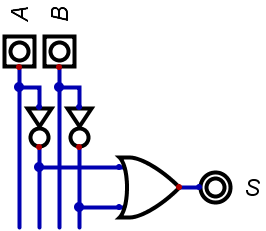
\includegraphics[scale=0.5]{Q4.png}
	\captionof{figure}{Circuit logique à étudier}
\end{minipage}

\begin{table}[!htb]
    \caption*{Tables de vérité}
    \begin{minipage}{.33\linewidth}
      \caption{}
      \centering
        \begin{tabular}{|c|c|c|}
		\hline 
		A & B & S \\ 
		\hline 
		0 & 1 & 1 \\ 
		\hline 
		0 & 1 & 0 \\ 
		\hline 
		0 & 1 & 1 \\ 
		\hline 
		0 & 1 & 0 \\ 
		\hline 
		\end{tabular} 
    \end{minipage}%
    \begin{minipage}{.33\linewidth}
      \centering
        \caption{}
        \begin{tabular}{|c|c|c|}
		\hline 
		A & B & S \\ 
		\hline 
		0 & 0 & 1 \\ 
		\hline 
		0 & 1 & 1 \\ 
		\hline 
		1 & 0 & 1 \\ 
		\hline 
		1 & 1 & 0 \\ 
		\hline 
		\end{tabular} 
    \end{minipage}
    \begin{minipage}{.33\linewidth}
      \centering
        \caption{}
        \begin{tabular}{|c|c|c|}
		\hline 
		A & B & S \\ 
		\hline 
		0 & 0 & 1 \\ 
		\hline 
		0 & 1 & 0 \\ 
		\hline 
		1 & 0 & 0 \\ 
		\hline 
		1 & 1 & 1 \\ 
		\hline 
		\end{tabular} 
    \end{minipage}  
\end{table}

\begin{table}[!htb]
  \caption*{}
    \begin{minipage}{.33\linewidth}
      \centering
        \caption{}
        \begin{tabular}{|c|c|c|}
		\hline 
		A & B & S \\ 
		\hline 
		0 & 0 & 0 \\ 
		\hline 
		0 & 1 & 1 \\ 
		\hline 
		1 & 0 & 1 \\ 
		\hline 
		1 & 1 & 0 \\ 
		\hline 
		\end{tabular} 
    \end{minipage}     
    \begin{minipage}{.33\linewidth}
      \centering
        \caption{}
        \begin{tabular}{|c|c|c|}
		\hline 
		A & B & S \\ 
		\hline 
		0 & 0 & 1 \\ 
		\hline 
		0 & 1 & 0 \\ 
		\hline 
		1 & 0 & 0 \\ 
		\hline 
		1 & 1 & 0 \\ 
		\hline 
		\end{tabular} 
    \end{minipage} 
\end{table}

\end{document}